\documentclass[a4paper,11pt]{article}
\usepackage{amssymb}
\usepackage[polish]{babel}
\usepackage[utf8]{inputenc}

\usepackage[T1]{fontenc}
\usepackage{graphicx}
\usepackage{anysize}
\usepackage{enumerate}
\usepackage{times}
\usepackage{geometry}
\usepackage{amsthm}
\usepackage{pgfplots}
\usepackage{amsmath}
\usepackage{mathtools}
\usepackage{amssymb}
\usepackage{multirow}
\usepackage{changepage}
\usepackage{pbox}

\marginsize{3cm}{3cm}{1.5cm}{1.5cm}
\sloppy

\begin{document}
\begin{table}[ht]
\centering
\hspace*{-1cm}
\begin{tabular}{lllllll}
\cline{1-6}
\multicolumn{1}{|c|}{\begin{tabular}[c]{@{}c@{}}EAIiIB\\ Informatyka\end{tabular}}              & \multicolumn{2}{l|}{\begin{tabular}[c]{@{}l@{}}Aleksander Lisiecki\\ Natalia Materek\end{tabular}}                                                                                                & \multicolumn{1}{c|}{\begin{tabular}[c]{@{}c@{}}Rok\\ II\end{tabular}}          & \multicolumn{1}{c|}{\begin{tabular}[c]{@{}c@{}}Grupa\\ 2\end{tabular}}            & \multicolumn{1}{c|}{\begin{tabular}[c]{@{}c@{}}Zespół\\ 6\end{tabular}}      &  \\ \cline{1-6}
\multicolumn{1}{|c|}{\begin{tabular}[c]{@{}c@{}}Pracownia\\ FIZYCZNA\\ WFiIS AGH\end{tabular}} & \multicolumn{4}{l|}{\begin{tabular}[c]{@{}l@{}}Temat:\\ \textbf{\textit{Współczynnik załamania ciał stałych}} \end{tabular}}                                                                                                                                                                                                                                            & \multicolumn{1}{c|}{\begin{tabular}[c]{@{}c@{}}Nr ćwiczenia:\\ 51\end{tabular}} &  \\ \cline{1-6}
\multicolumn{1}{|l|}{\begin{tabular}[c]{@{}c@{}}Data wykonania:\\ 16.01.2017\end{tabular}}      & \multicolumn{1}{c|}{\begin{tabular}[c]{@{}c@{}}Data oddania:\\ 18.01.2017\end{tabular}} & \multicolumn{1}{l|}{\begin{tabular}[c]{@{}l@{}}Zwrot do poprawki:\\ \phantom{data poprawki}\end{tabular}} & \multicolumn{1}{l|}{\begin{tabular}[c]{@{}l@{}}Data oddania:\\  \phantom{data oddania}\end{tabular}} & \multicolumn{1}{l|}{\begin{tabular}[c]{@{}l@{}}Data zaliczenia:\\  \phantom{data zaliczenia}\end{tabular}} & \multicolumn{1}{l|}{\begin{tabular}[c]{@{}l@{}}OCENA:\\ \phantom{ocena}\end{tabular}}       &  \\ \cline{1-6}
                                                                                               &                                                                                         &                                                                                     &                                                                                &                                                                                   &                                                                               & 
\end{tabular}
\end{table}

\begin{center}
\begin{LARGE}
\textbf{Ćwiczenie nr 51: Współczynnik załamania ciał stałych}
\end{LARGE}
\end{center}

\section{Cel ćwiczenia}
\indent Wyznaczenie współczynnika załamania światła dla ciał stałych metodą mikroskopu. 
Zbadanie zależności współczynnika załamania od długości fali.

\section{Wstęp}
\indent Załamanie światła na granicy dwóch ośrodków przeźroczystych. Promień padający biegnący w~pierwszym ośrodku pada na granicę ośrodków po czym zmienia kierunek, i jako promień złamany biegnie w ośrodku drugim.	
Wiązka światła ulega załamaniu, gdy przechodzi z jednego ośrodka do drugiego o innych własnościach optycznych.
\begin{equation}
\frac{\sin{\alpha}}{\sin{\beta}} = \frac{V_1}{V_2}
\end{equation}
gdzie 
\begin{description}
\item [$\alpha$] kąt padania
\item [$\beta$] kąt załamania
\item [$V_{1}$] prędkość światła w ośrodku pierwszym $\left[\frac{m}{s}\right]$
\item [$V_{2}$] prędkość światła w ośrodku drugim $\left[\frac{m}{s}\right]$
\end{description}

\indent Stosunek sinusa kąta padania do sinusa kąta załamania, zwany współczynnikiem załamania n~ośrodka 2 względem ośrodka 1, jest równy stosunkowi prędkości rozchodzenia się fali w ośrodku 1 do prędkości rozchodzenia się fali w ośrodku 2. W obu ośrodkach promień fali padającej, promień fali załamanej i prosta prostopadła do granicy ośrodków leżą w jednej płaszczyźnie. Prawo załamania zostało sformułowane przez Snelliusa w XVII wieku. \\
\begin{equation}
n = \frac{\sin{\alpha}}{\sin{\beta}} = \frac{V_1}{V_2} = \frac{n_2}{n_1}
\end{equation}
gdzie 
\begin{description}
\item [$n$] względny współczynnik załamania światła ośrodka 2 względem ośrodka 1
\item [$n_{1}$] bezwzględny współczynnik załamania światła dla ośrodka 1 wynoszący $n_{1}=\frac{c}{v_1}$
\item [$n_{2}$] bezwzględny współczynnik załamania światła dla ośrodka 2 wynoszący $n_{2}=\frac{c}{v_2}$
\item [$c$] prędkość światła w próżni $\left[\frac{m}{s}\right]$
\end{description}

W płytce równoległościennej zachodzi:
\begin{equation}
\label{wzor:n}
n = \frac{\sin{\alpha}}{\sin{\beta}} = \frac{d}{h}
\end{equation}
gdzie 
\begin{description}
\item [$d$] grubość rzeczywista płytki równoległościennej [$mm$]
\item [$h$] grubość pozorna płytki równoległościennej [$mm$]
\end{description}

\begin{figure}[ht]
	\centering
	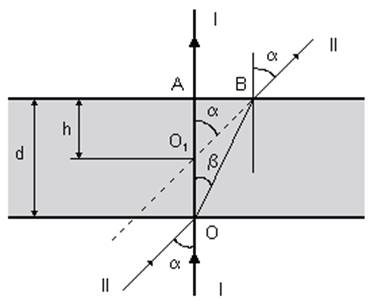
\includegraphics[width=90mm]{image006.jpg}
	\caption{Powstanie  pozornego  obrazu  $O_{1}$ punktu  $O$  leżącego  na  dolnej  powierzchni płytki płaskorównoległej. }
\end{figure}

\indent W skutek załamania wiązki światła odległości przedmiotów umieszczonych w środowisku optycznie gęstszym obserwowane z powietrza wydają się mniejsze. Przykładami mogą być szyba, która wydaje się być cieńsza niż w rzeczywistości lub choćby nawet przedmioty w wodzie, które wydają się być bliżej tafli. Widać to wyraźnie na przykładzie płytki płaskorównoległej:
Promień $OB$ tworzy z prostopadłą wewnątrz szkła kąt $\beta$, a w powietrzu kąt $\alpha$ (wskutek załamania $\alpha > \beta$). Obserwowane promienie, które wychodzą z płytki są rozbieżne, a ich przedłużenia przecinają się w punkcie $O_1$ tworząc obraz pozorny. Rzeczywista grubość płytki to: $d = AO$, natomiast $h = AO_1$ stanowi pozorną grubość płytki płaskorównoległej.


\section{Układ pomiarowy}
\begin{enumerate}
\item Mikroskop wyposażony w czujnik mikrometryczny i nasadkę krzyżową.
\item Śruba mikrometryczna. 
\item Płytka szklana i z pleksiglasu.
\end{enumerate}

\section{Przebieg doświadczenia}
\begin{enumerate}
\item Odczytanie położenia $a_{g}$ z wskazówki czujnika mikrometrycznego po uzyskaniu ostrego obrazu śladu na górnej powierzchni płytki (przez przesunięcie stolika mikroskopu).
\item Odczytanie położenia $a_{d}$ z wskazówki czujnika mikrometrycznego po uzyskaniu ostrego obrazu śladu na dolnej powierzchni płytki(przez przesunięcie stolika mikroskopu).
\item Policzenie grubości pozornej $h = a_{d} - a_{g}$
\item Powtórzenie kroków 1 i 3 dziesięciokrotnie dla każdej płytki oraz dla płytki z filtrem czerwonym/ niebieskim.
\item Obliczenie średniej grubości pozornej ze wzoru:
\begin{equation}
\label{wzor:hśr}
h_{\text{śr}} = \frac{\sum_{i=1}^{10}h_{i}}{10}
\end{equation}
gdzie $h_{i}$ to kolejne pomiary $h$
\item Obliczenie względnego współczynnika załamania światła korzystając ze wzoru {\ref{wzor:n}}.
\item Obliczenie niepewności pomiarowych.
\end{enumerate}

\section{Wyniki pomiarów}

	\begin{adjustwidth}{-1cm}{}
\def\arraystretch{1.3}
\begin{center}
	\begin{tabular}{|c|c|c|c|}
	
		\hline
		\multicolumn{4}{|l|}{\begin{tabular}{l} Materiał: szkło Grubość rzeczywista: $d =2,73$ [mm]\\ niepewność $u(d)=0,0058$ [mm] \end{tabular}}\\
		\hline
		
		\multirow{3}{*}{Lp.} & \multicolumn{2}{|c|}{Wskazanie czujnika} & \begin{tabular}{c}Grubość \\pozorna\end{tabular}  \\ \cline{2-4}
		& \parbox[c]{1.8 cm}{\centering $a_{d}$}  & $a_{g}$ & $h=a_{d}-a_{g}$  \\ \cline{2-4}
		& [mm] & [mm] & [mm] \\ 
		
		\hline
		1. & 6,03 & 4,19 & 1,84\\
		\hline
		2. & 6,11 & 4,03 & 2,08\\
		\hline
		3. & 6,07 & 4,03 & 2,04\\
		\hline
		4. & 6,02 & 4,23 & 1,79\\
		\hline
		5. & 6,02 & 4,23 & 1,79\\
		\hline
		6. & 5,85 & 4,00 & 1,85\\
		\hline
		7. & 5,82 & 3,98 & 1,84\\
		\hline
		8. & 5,87 & 4,02 & 1,85\\
		\hline
		9. & 5,87 & 4,01 & 1,86\\
		\hline
		10.& 5,86 & 4,03 & 1,83\\
		\hline
		\multicolumn{2}{c|}{}&\begin{tabular}{c}Wartość \\ średnia $h{\text{śr}}$ [$mm$] \end{tabular} & 1,88 \\
		\cline{3-4}
		\multicolumn{2}{c|}{}&\begin{tabular}{c}Niepewność $u(h)$ [$mm$]\end{tabular}& ...\\
		\cline{3-4}
	\end{tabular}
	\end{center}
\end{adjustwidth}


\begin{adjustwidth}{-1cm}{}
\def\arraystretch{1.3}
\begin{center}
	\begin{tabular}{|c|c|c|c|}
	
		\hline
		\multicolumn{4}{|l|}{\begin{tabular}{l} Materiał: pleksiglas Grubość rzeczywista: $d =1,50$ [mm]\\ niepewność $u(d)=0,0058$ [mm] \end{tabular}}\\
		\hline
		
		\multirow{3}{*}{Lp.} & \multicolumn{2}{|c|}{Wskazanie czujnika} & \begin{tabular}{c}Grubość \\pozorna\end{tabular}  \\ \cline{2-4}
		& \parbox[c]{1.8 cm}{\centering $a_{d}$}  & $a_{g}$ & $h=a_{d}-a_{g}$  \\ \cline{2-4}
		& [mm] & [mm] & [mm] \\ 
		
		\hline
		1. & 1,09 & 0,00 & 1,09\\
		\hline
		2. & 1,08 & 0,00 & 1,08\\
		\hline
		3. & 1,10 & 0,00 & 1,10\\
		\hline
		4. & 1,05 & 0,00 & 1,05\\
		\hline
		5. & 1,07 & 0,00 & 1,07\\
		\hline
		6. & 1,13 & 0,00 & 1,13\\
		\hline
		7. & 1,11 & 0,00 & 1,11\\
		\hline
		8. & 1,09 & 0,00 & 1,09\\
		\hline
		9. & 1,07 & 0,00 & 1,07\\
		\hline
		10.& 1,10 & 0,00 & 1,10\\
		\hline
		\multicolumn{2}{c|}{}&\begin{tabular}{c}Wartość \\ średnia $h{\text{śr}}$ [$mm$] \end{tabular} & 1,09 \\
		\cline{3-4}
		\multicolumn{2}{c|}{}&\begin{tabular}{c}Niepewność $u(h)$ [$mm$]\end{tabular}& ...\\
		\cline{3-4}
	\end{tabular}
	\end{center}
\end{adjustwidth}
	
	
\begin{adjustwidth}{-1cm}{}
\def\arraystretch{1.3}
\begin{center}
	\begin{tabular}{|c|c|c|c|}
	
		\hline
		\multicolumn{4}{|l|}{\begin{tabular}{l} Materiał: szkło, filtr czerwony Grubość rzeczywista: $d =2,73$ [mm]\\ niepewność $u(d)=0,0058$ [mm] \end{tabular}}\\
		\hline
		
		\multirow{3}{*}{Lp.} & \multicolumn{2}{|c|}{Wskazanie czujnika} & \begin{tabular}{c}Grubość \\pozorna\end{tabular}  \\ \cline{2-4}
		& \parbox[c]{1.8 cm}{\centering $a_{d}$}  & $a_{g}$ & $h=a_{d}-a_{g}$  \\ \cline{2-4}
		& [mm] & [mm] & [mm] \\ 
		
		\hline
		1. & 5,77 & 4,04 & 1,73\\
		\hline
		2. & 5,90 & 3,98 & 1,92\\
		\hline
		3. & 5,95 & 3,95 & 2,00\\
		\hline
		4. & 5,73 & 3,98 & 1,75\\
		\hline
		5. & 5,76 & 4,00 & 1,76\\
		\hline
		6. & 5,85 & 4,01 & 1,84\\
		\hline
		7. & 5,90 & 3,98 & 1,92\\
		\hline
		8. & 5,98 & 4,03 & 1,95\\
		\hline
		9. & 6,01 & 4,05 & 1,98\\
		\hline
		10.& 6,03 & 4,09 & 1,94\\
		\hline
		\multicolumn{2}{c|}{}&\begin{tabular}{c}Wartość \\ średnia $h{\text{śr}}$ [$mm$] \end{tabular} & 1,80 \\
		\cline{3-4}
		\multicolumn{2}{c|}{}&\begin{tabular}{c}Niepewność $u(h)$ [$mm$]\end{tabular}& ...\\
		\cline{3-4}
	\end{tabular}
	\end{center}
\end{adjustwidth}
	
	
\begin{adjustwidth}{-1cm}{}
\def\arraystretch{1.3}
\begin{center}
	\begin{tabular}{|c|c|c|c|}
	
		\hline
		\multicolumn{4}{|l|}{\begin{tabular}{l} Materiał: pleksiglas, filtr niebieski Grubość rzeczywista: $d =1,50$ [mm]\\ niepewność $u(d)=0,0058$ [mm] \end{tabular}}\\
		\hline
		
		\multirow{3}{*}{Lp.} & \multicolumn{2}{|c|}{Wskazanie czujnika} & \begin{tabular}{c}Grubość \\pozorna\end{tabular}  \\ \cline{2-4}
		& \parbox[c]{1.8 cm}{\centering $a_{d}$}  & $a_{g}$ & $h=a_{d}-a_{g}$  \\ \cline{2-4}
		& [mm] & [mm] & [mm] \\ 
		
		\hline
		1. & 1,07 & 0,00 & 1,07\\
		\hline
		2. & 1,06 & 0,00 & 1,06\\
		\hline
		3. & 1,08 & 0,00 & 1,08\\
		\hline
		4. & 1,00 & 0,00 & 1,00\\
		\hline
		5. & 1,02 & 0,00 & 1,02\\
		\hline
		6. & 1,05 & 0,00 & 1,05\\
		\hline
		7. & 1,04 & 0,00 & 1,04\\
		\hline
		8. & 1,05 & 0,00 & 1,05\\
		\hline
		9. & 1,06 & 0,00 & 1,06\\
		\hline
		10.& 1,01 & 0,00 & 1,01\\
		\hline
		\multicolumn{2}{c|}{}&\begin{tabular}{c}Wartość \\ średnia $h{\text{śr}}$ [$mm$] \end{tabular} & 1,01 \\
		\cline{3-4}
		\multicolumn{2}{c|}{}&\begin{tabular}{c}Niepewność $u(h)$ [$mm$]\end{tabular}& ...\\
		\cline{3-4}
	\end{tabular}
	\end{center}
\end{adjustwidth}

\section{Obliczenia}
\subsection{Obliczenie wartości współczynnika n}
\indent Aby obliczyć współczynnik załamania $n$ dla każdej próbki korzystamy ze wzoru {\ref{wzor:n}}. \\

\textbf{Współczynnik załamania dla szkła bez filtra:}
$$ n = \frac{2,73}{1,88} \approx ... $$
\textbf{Współczynnik załamania dla szkła z czerwonym filtrem:}
$$ n = \frac{2,73}{1,80} \approx ... $$
\textbf{Współczynnik załamania dla pleksiglasu bez filtru:}
$$ n = \frac{1,50}{1,09} \approx ... $$
\textbf{Współczynnik załamania dla pleksiglasu z niebieskim filtrem:}
$$ n = \frac{1,50}{1,04} \approx ... $$

\subsection{Niepewność wyznaczenia grubości płytki}
Niedokładność pomiaru śrubą mikrometryczną wynosi $0,01 mm$ gdyż jest to najmniejsza możliwa do odczytania wartość na śrubie mikrometrycznej.\\
Więc niepewność pomiaru grubości płytki typu B przyjmujemy:
$$u(d)= \frac{0,01}{\sqrt{3}} \approx 0,0058 [mm]$$

\subsection{Niepewność wyznaczenia grubości pozornej}
Do obliczenia niepewności typu A dla grubości pozornej $h$ korzystamy ze wzoru:
$$u(h) = \sqrt{\frac{\sum(h_{i}-\overline{h})^{2}}{n(n-1)}}$$

gdzie 
\begin{description}
\item [$u(h)$] niepewność wyznaczenia średniej grubości pozornej [$mm$]
\item [$n$] liczba pomiarów
\item [$h_{i}$] grubość pozorna wyznaczona w $i$ - tym pomiarze [$mm$]
\end{description}

\textbf{Dla szkła bez filtru:}
$$u(h)=\displaystyle \sqrt{\frac{(1,84-1,88)^{2}+\cdots +(1,83-1,88)^{2}}{10(10-1)}}~mm= ...~mm$$	

\textbf{Dla szkła z czerwonym filtrem:}
$$u(h)=\displaystyle \sqrt{\frac{(1,73-1,80)^{2}+\cdots +(1,94-1,80)^{2}}{10(10-1)}}~mm= ...~mm$$	

\textbf{Dla pleksiglasu bez filtru:}
$$u(h)=\displaystyle \sqrt{\frac{(1,09-1,09)^{2}+\cdots +(1,11-1,09)^{2}}{10(10-1)}}~mm= ...~mm$$

\textbf{Dla pleksiglasu z niebieskim filtrem:}
$$u(h)=\displaystyle \sqrt{\frac{(1,07-1,04)^{2}+\cdots +(1,01-1,04)^{2}}{10(10-1)}}~mm= ...~mm$$

\subsection{Niepewność wyznaczenia współczynnika załamania}
Następnie wyznaczamy niepewność obliczonego współczynnika załamania światła z prawa przenoszenia niepewności:
$$ u(n) =\sqrt{\bigg(\frac{\partial n}{\partial d}u(d)\bigg)^2+\bigg(\frac{\partial n}{\partial h}u(h)\bigg)^2} = \sqrt{\bigg(\frac{1}{h}u(d)\bigg)^2+\bigg(\frac{-d}{h^2}u(h)\bigg)^2}$$
gdzie 
\begin{description}
\item [$u(n)$]
\item [$u(d)$]
\item [$u(h)$]
\end{description}

\textbf{Dla szkła bez filtru:}
$$ u(n) = \sqrt{\bigg(\frac{1}{...}\cdot 0,0058\bigg)^2+\bigg(\frac{...} {...^2}\cdot ...\bigg)^2} = ...$$

\textbf{Dla szkła z czerwonym filtrem:}
$$ u(n) = \sqrt{\bigg(\frac{1}{...}\cdot 0,0058\bigg)^2+\bigg(\frac{...} {...^2}\cdot ...\bigg)^2} = ...$$

\textbf{Dla pleksiglasu bez filtru:}
$$ u(n) = \sqrt{\bigg(\frac{1}{...}\cdot 0,0058\bigg)^2+\bigg(\frac{...} {...^2}\cdot ...\bigg)^2} = ...$$

\textbf{Dla pleksiglasu z niebieskim filtrem:}
$$ u(n) = \sqrt{\bigg(\frac{1}{...}\cdot 0,0058\bigg)^2+\bigg(\frac{...} {...^2}\cdot ...\bigg)^2} = ...$$

\section{Porównanie z wartościami tabelarycznymi}
\begin{table}[!h]
\begin{tabular}{|c|c|c|}
\hline
rodzaj materiału & $n$ zmierzone & $n$ tablicowe \\
\hline
szkło (bez filtru) & & \\
\hline
szkło (filtr czerwony) & & \\
\hline
pleksiglas (bez filtru) & & \\
\hline
pleksiglas (filtr niebieski) & & \\
\hline
\end{tabular}
\end{table}
\section{Wnioski}
\begin{enumerate}
\item cos tam
\end{enumerate}
\end{document}